\def\theTopic{Normal Proportions }
\def\dayNum{22 }


\begin{center}
   {\Large\bf  Proportions}
 \end{center}

If we mix 40 blue balls and 80 gold balls together in a jar and draw
out 30 at random with replacement, the sampling distribution for the
proportion of blue balls in a sample of size 30 looks like this:

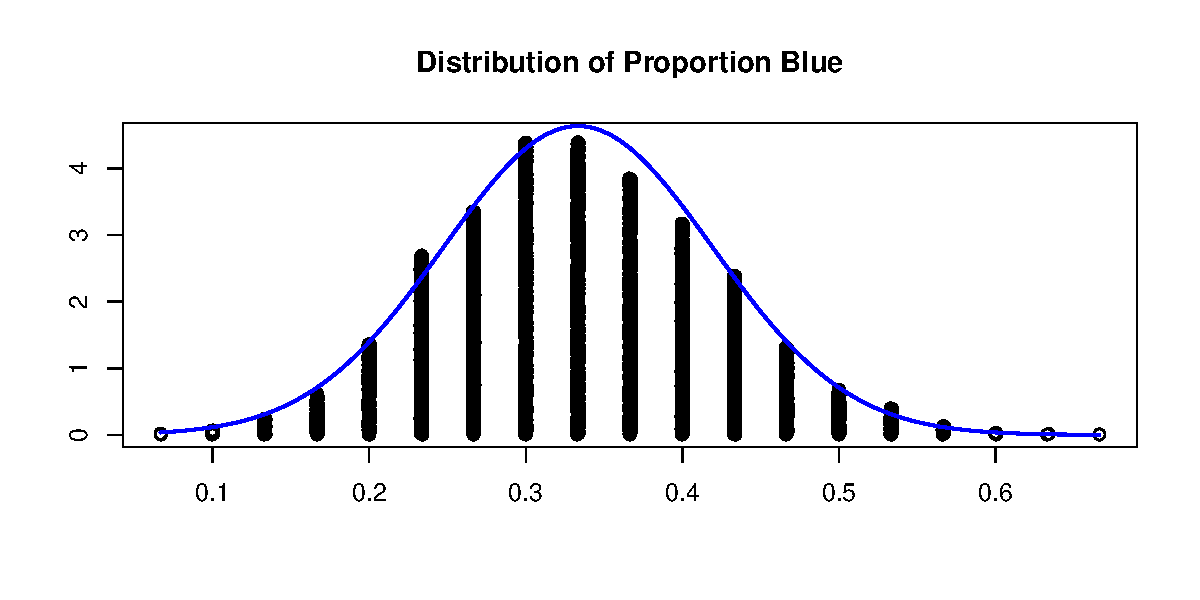
\includegraphics[width=.8\linewidth]{../../plots/sample1.pdf}

Each of 5000 dots came from a computer simulation in which we sampled
30 draws from the container at random with replacement, and computed
the proportion of blue balls in the simulated sample.  The density
curve shown on top of the dots is the density of the normal
distribution with the same center and spread as the distribution of
dots.

With modern computers, we can easily simulate random draws five or ten
thousand times, and/or we can easily obtain probabilities from the
normal distribution.  Both are valid tools, and each method can give
us the p-values and confidence intervals that we need.  We did the
simulation approach first because it allowed us to bypass two weeks of
more theoretical probability and quickly get to the meat of this
course -- statistical inference.  Now it's time to see how the other
approach works, and we'll continue to emphasize the interpretation of
p-values and confidence intervals.  


%% <<sample1, echo=FALSE, fig.width=6,fig.height=4,out.width='.75\\linewidth'>>=
%%   reps <- 5000
%%   n <- 30
%%   p <- 1/3
%%   blueProp <- rbinom(reps,n,p) / n
%%   x <- sort(blueProp)
%%   y <- unlist(tapply(x, x, function(z) 1:length(z))) /reps / diff(range(x)) * (length(unique(x))-1.5)
%% ##  rescale to meet normal density
%%   plot(jitter(x, .1), y, main = "Distribution of Proportion Blue", xlab = "", ylab = "")
%%   curve(dnorm(x,p,sqrt(p*(1-p)/n)),add=TRUE,col=4,lwd=2)
 %  dev.copy2pdf(file="plots/sample1.pdf",height=4,width=8)

% # summary(nlme::RatPupWeight$weight)
% #   Min. 1st Qu.  Median    Mean 3rd Qu.    Max. 
% #  3.680   5.650   6.055   6.081   6.398   8.330 
% # sd(nlme::RatPupWeight$weight)
% #[1] 0.6474272
% # locator(1) #$y 0.6190716
 
  %# summary(faraway::aatemp$temp)
 %#   Min. 1st Qu.  Median    Mean 3rd Qu.    Max. 
 %#  43.41   46.78   47.73   47.74   48.64   51.89 
 %# sd(faraway::aatemp$temp) ] 1.526413
 %# locator(1)$y[1] 0.2773441

%# sd(nlme::Oxboys$height)
%#[1] 9.10321
 % #summary(nlme::Oxboys$height)
 % #  Min. 1st Qu.  Median    Mean 3rd Qu.    Max. 
 % # 126.2   143.8   149.5   149.5   155.5   174.8 
 % #locator(1) # 0.04889153
 %
 % par(mfrow=c(1,3))
 % hist(nlme::RatPupWeight$weight,breaks=20,probability=TRUE, main=" ",
 % xlab = "Weight")
 % curve(dnorm((x-6)/0.647)/.3989*.63,col=4,add=TRUE)
 % hist(faraway::aatemp$temp,breaks=18,probability=TRUE, main=" ", xlab
 % = "Temperature")
 % curve(dnorm((x-47.6)/1.526)/.3989*.26,col=4,add=TRUE)
 % hist(nlme::Oxboys$height,breaks=18,probability=TRUE, main=" ", xlab =
 % "Height (cm)")
 % curve(dnorm((x-149.5)/9.1)/.3989*.047,col=4,add=TRUE)
 % dev.copy(png, file="plots/normals.png",height=300,width=800);dev.off()
%% @ 
      
%% 
  
We can use spinners and coin flips to simulate the distribution
of a proportion.  From that distribution we use the standard
deviation of the resampled points to get the standard error of
$\phat$.  We added two standard errors 
to -- and subtracted two standard errors from -- the point estimate to build our
confidence interval.  In order to use the normal distribution instead of a
simulation,  we need this formula for standard error of the sample
proportion: 
    $$ SE(\widehat{p}) = \sqrt{\widehat{p}(1-\widehat{p})/n} $$
 We can then multiply $SE(\widehat{p})$ by the appropriate $z^*$
 value from the normal distribution to get whatever confidence
 level we need.  Setting margin of error to $2 SE$ was a good
 approximation for a 95\% confidence interval, but you'll see in
 this web app that a more precise value is 1.96 $SE$'s on each
 side.


{\bf Notation:} We have two ways to describe the same measure
of spread. For any distribution, we can compute the spread, or
standard deviation of the sampled values.  When we talk about the
sampling distribution of a statistic, we can  refer to the
standard deviation of the sampling distribution because it is a
distribution, so it has some ``spread''.   However, we prefer
to talk about the ``Standard Error'' (or SE) of the statistic.  We'll
be able to show the difference better when we look at the mean of a
continuous variable, so we'll come back to this. 

When we write $SE(estimate)$ as in $SE(\phat)$ or $SE(\xb)$, we {\bf
  do not} mean to multiply $SE$ by the estimate. This is notation to
say SE is a function which we apply to the estimate. We read it as
``standard error of $\ldots$'' just like when we take log of $x$ we
write $\log(x)$.  

  \begin{center}
    {\bf Confidence Intervals}
  \end{center}

The general form is 
$$ \mbox{estimate} \pm z^* SE(\mbox{estimate})$$
or for proportions:
$$ \widehat{p} \pm z^*\sqrt{\widehat{p}(1-\widehat{p})/n}$$

To build confidence intervals, we use the same $z^*$ values over and
over again.  Go to the web app
\url{http://shiny.math.montana.edu/jimrc/IntroStatShinyApps}, select
\fbox{Normal Distribution} under \fbox{One Categ} and  put
confidence levels 0.80, 0.90, $\ldots$, 0.99 into the probability box
(one at a time).  Change \fbox{Lower} to
\fbox{Center} to get the confidence limits. Write them into this
table.  \vspace{1cm}
 
\begin{students}
   \begin{tabular}{l|rrrrr}
    Confidence level: &  \hspace{1cm}80\% &  \hspace{1cm}90\% &  \hspace{1cm}95\% & \hspace{1cm} 98\% & \hspace{1cm} 99\% \\ \hline
    $z^*$ cutoff  &  &  & 1.96 &  & 
  \end{tabular}
\end{students}
\begin{key}
   \begin{tabular}{l|rrrrr}
    Confidence level: &  \hspace{1cm}80\% &  \hspace{1cm}90\% &  \hspace{1cm}95\% & \hspace{1cm} 98\% & \hspace{1cm} 99\% \\ \hline
    $z^*$ cutoff  &1.282  &1.645  & 1.96 &2.326& 2.575
  \end{tabular}
\end{key}


Let's try it out:  
 \begin{enumerate}
   \item 
     In a survey of  2142 American adults, 1221 gave the opinion that
     college is a ``poor to fair'' value.  We want to estimate the
     proportion of all American adults with that opinion using a 99\%
     confidence interval.  
     \begin{enumerate}
     \item Compute $\widehat{p}$ for these data. 
\begin{students}
        \vspace{1cm}        
\end{students}

\begin{key}
  {\it 0.57 }
\end{key}
     \item \label{propSE} Compute the standard error of the estimate.
\begin{students}
        \vspace{1cm}        
\end{students}

\begin{key}
  {\it $ \sqrt{0.57\times 0.43/2142} = 0.0107$ }
\end{key}

     \item Find the margin of error and compute a 99\% CI using the
       multiplier you found   above.
\begin{students}
        \vspace{1cm}        
\end{students}

\begin{key}
  {\it ME = $ 2.575 \times 0.0107 = 0.02755$, CI: $0.57 \pm  0.0276 = (0.542, 0.598 )$ }
\end{key}

     \item If we use resampling to create a 99\% bootstrap percentile
       confidence interval, it is $(0.542, 0.597)$ and the {\sf SE} in
       the plot is 0.011.  Which interval is narrower? 
\begin{students}
        \vspace{1cm}        
\end{students}

\begin{key}
  {\it Bootstrap is a hair narrower.}
\end{key}

     How similar is the standard error from \ref{propSE} to the
     bootstrap SE?        
\begin{students}
        \vspace{2cm}         
\end{students}

\begin{key}
  {\it Very close. Off just by round off error?}
\end{key}

\item Interpret the interval in the context of this problem.  What do
  we mean by the word ``confidence''?    
\begin{students}
        \vspace{3cm}        
\end{students}

\begin{key}
  {\it We are 99\% confident that the true proportion of US adults
  who thought that college was a poor to fair investment is within the
interval (0.542, 0.597). Our confidence is in the process: when we use
this method over and over take a sample and compute a 99\% CI from it,
in the long run, 99\% of those intervals will contain the true parameter.}
\end{key}
     \end{enumerate}
   \end{enumerate}
 

     \begin{center}
       {\large\bf Assumptions}
     \end{center}

  To do any statistical analysis, we must make some assumptions.  We
  should always check to see if the data indicate a violation of an
  assumption. For the methods used before today we need:
     \begin{itemize}
     \item A population of size at least $10n$. 
       (If a sample is a really large part of the population, our
       methods over-estimate sampling variation.) 
     \item Representative sample. 
     \item Independent trials (one outcome has no effect on another).  
     \end{itemize}
   
  Using normal distributions adds another assumption:
   \begin{itemize}
     \item Large enough sample size to expect at least 10
       successes   and  at least 10  failures.  If you are building a
       confidence interval, just make sure the counts are over 10. If
       you are conducting a hypothesis test, we need $np_0\geq 10$ and
       $n(1-p_0) \geq 10$. 
     \end{itemize}\vspace{1cm}


   \begin{enumerate}
     \setcounter{enumi}{1}
   \item In an earlier assignment  you checked to see if a roulette wheel was
     fair.  Were these assumptions met? The
     observer saw 3 ``Greens'' in 30 spins, and the  chance of
     green for a fair wheel is $2/38$. 
     \begin{enumerate}
        \item Is population size at least $10n$ ($n = 30$)? 
          Hint: How many spins are possible?    
\begin{students}
        \vspace{.7cm}        
\end{students}
\begin{key}
  {\it  An almost infinite number, so assumption is met.}
\end{key}
        \item Representative sample?   
\begin{students}
        \vspace{.7cm}        
\end{students}

\begin{key}
  {\it  One spin should be like another, so I don't question this  assumption.}
\end{key}
        \item Independent trials?   
\begin{students}
        \vspace{.7cm}        
\end{students}

\begin{key}
  {\it  If there is no cheating, this assumption is met.}
\end{key}
        \item At least 10 successes? at least 10 failures?   
\begin{students}
        \vspace{.7cm}        
\end{students}

\begin{key}
  {\it  Not met. 27 ``Failures'' and only 3 ``Successes''.}
\end{key}
     \end{enumerate}


    \item In the Unit 1 Review you estimated the probability
      a kissing couple leans to the right from data in which 80 of 124
      couples did lean to the right. Let's check assumptions. 
  
     \begin{itemize}
        \item Is population size at least $10n$ ($n = 124$)? 
\begin{students}
        \vspace{.7cm}        
\end{students}

\begin{key}
  {\it  All couples, so assumption is met.}
\end{key}
        \item Representative sample?   
\begin{students}
        \vspace{1cm}        
\end{students}

\begin{key}
  {\it  Sort of random observations, so I hope this   assumption is met.}
\end{key}
        \item Independent trials?   
\begin{students}
        \vspace{1cm}        
\end{students}

\begin{key}
  {\it  Couple should act independently, so this assumption is met.}
\end{key}
        \item At least 10 successes? at least 10 failures?   
\begin{students}
        \vspace{1cm}        
\end{students}

\begin{key}
  {\it  Yes, $80>10$ and $44 > 10$}
\end{key}
     \end{itemize}
     \begin{enumerate}
     \item Now we'll build a 99\% confidence interval for the true
       proportion of couples leaning right when kissing using normal
       procedures. 
       \begin{enumerate}
       \item What is the sample statistic?  
\begin{students}
        \vspace{1cm}        
\end{students}

\begin{key}
  {\it  0.645}
\end{key}
       \item What is the standard error of $\widehat{p}$ for these
         data?   
\begin{students}
        \vspace{.7cm}        
\end{students}

\begin{key}
  {\it  $\sqrt{0.645 * 0.355 / 124} = 0.0430 $}
\end{key}
       \item From the table about two pages back, what $z^*$ values
         goes with 99\% confidence?   
       \end{enumerate}
\begin{students}
        \vspace{.7cm}        
\end{students}

\begin{key}
  {\it  2.576}
\end{key}
       \item Build the interval and interpret its meaning. 
\begin{students}
        \newpage
\end{students}

\begin{key}
 {\it $(0.534, 0.756)$.  We are 99\% confident that the true
    proportion of couples who lean right when kissing is between 53.4
    and 75.6\%. }
\end{key}
     \end{enumerate}
   \end{enumerate}

   \begin{center}
     {\large\bf   Hypothesis testing }
   \end{center}

 Reminder:  when we do hypothesis testing, we give the benefit
 of the doubt to: \underline{\hspace{1in}}.

 Our assumption of ``innocent until proven guilty'' changes the
 formula for standard error.  We plug in the null hypothesis value
 instead of the sample proportion, so when hypothesis testing: $
 SE(\widehat{p}) = \sqrt{p_0(1-p_0)/n}$. Secondly, instead of counting
 points as or more extreme than the observed statistic, we will use
 the normal distribution to compute the probabilities.  To do that, we
 need to convert the distance between $p_0$ and $\widehat{p}$ to ``standard
 deviation'' units by dividing by $SE(\widehat{p})$.  The complete
 formula is:
  $$ z = \frac{\widehat{p} - p_0}{SE(\widehat{p})} = 
         \frac{\widehat{p} - p_0}{\sqrt{p_0(1-p_0)/n}}$$
   
 We will illustrate with the ``Kissing on the Right'' data. As we did
 before, we will not assume which direction the alternative will
 take, but the null is that couples are equally likely to lean
 left or right. 
 
    \begin{enumerate}
\setcounter{enumi}{3}
    \item State null and alternative hypotheses in symbols and
      words.\\
      $H_0:$ 
\begin{students}
    \vspace{1.2cm}    \\
\end{students}
\begin{key} 
{\it $p = .5$.  Half of all couples lean right when kissing.}
\end{key}
$H_a:$
\begin{students}
    \vspace{.7cm}    \\
\end{students}

\begin{key} 
{\it $p \neq .5$.  The true proportion of couples leaning right when
  kissing is not one half.}
\end{key}
\item Compute the $SE(\widehat{p})$ using the null hypothesis value
  for $p$. 
\begin{students}
    \vspace{1cm}    \\
\end{students}

\begin{key} 
{\it $SE(\widehat{p}) = \sqrt{.5(.5)/124} = 0.0449$}
\end{key}

  \item Build the $z$ statistic by dividing the difference between
    $\widehat{p}$ and $p_0$ by $SE(\widehat{p})$. 
\begin{students}
    \vspace{1cm}    \\
\end{students}

\begin{key} 
{\it $z = \frac{.645 - .5}{0.0499} = 3.23$}
\end{key}

  \item Put the standardized $z$ value into the web app 
    \url{http://shiny.math.montana.edu/jimrc/IntroStatShinyApps},
    \fbox{One Categ} -- \fbox{Normal Distribution} and ask for
    the \fbox{Extremes}.  What part of the plot is shaded?  What is
    the (total) p-value and how strong is this evidence against $H_0$?  
\begin{students}
    \vspace{1cm}    \\
\end{students}

\begin{key} 
{\it $2 \times .001 = .002$  This is  very strong evidence against the
  null. }
\end{key}


\item Report the strength of evidence.  At the $\alpha = .01$ level of
  significance, what do you decide to do with $H_0$?  What is your
  conclusion?
\begin{students}
    \newpage
\end{students}

\begin{key} 
{\it We  reject $H_0$
  at the 1\% significance level.  We conclude that the true proportion of
  couples who lean right when kissing is over 0.50.}
\end{key}

\end{enumerate}

\begin{center}
  {\large \bf Rock, Paper, Scissors}
\end{center}

A student played a game of ``Rock, Paper, Scissors'' with each of 120
inexperienced players and found that 55 of his opponents first chose
``Rock''.  We want to test to see if the three options are equally
likely and to build a confidence interval for the true proportion to
pick ``Rock''.

\begin{enumerate}
 \setcounter{enumi}{8}
 \item  Check the assumptions.
\begin{students}
\\   \vspace{2cm}    
\end{students}

\begin{key} 
 {\it There is a huge population of potential first time players, so
  we have less than 10\% of the population.  We'd like to know how the
  opponents were selected. We can't assume they are representative,
  and if they watched some of his earlier games, they might be
  influenced in their 
  choices. We cannot assume independence from the data provided. We do
have large enough sample size to use normality because $55 > 10$ and
$120-55 = 65>0$ (for CI) and $np_0 = 120\times 1/3 = 40>10$ (for
hypothesis test).}
\end{key}
\item Although you should have identified some possible problems with
  the assumptions, we will go ahead with the normal theory based
  inference. Compute $\widehat{p}$ and its SE for a confidence
  interval.
\begin{students}
    \vspace{1cm}    \\
\end{students}

\begin{key} 
{\it $\widehat{p} = 55/120 = 0.458$ with SE = $\sqrt{.458(.542)/120} =
  0.0455$}
\end{key}
\item Build a 90\% confidence interval for the true mean proportion of
  first time players who pick ``Rock''.
\begin{students}
    \vspace{1cm}    \\
\end{students}

\begin{key} 
{\it $0.458 \pm 1.645 \times 0.0455 = (0.383, 0.533)$}
\end{key}
\item Now switch to thinking of a hypothesis test using ``random
  guessing'' as the null model.  What are the null and alternative
  hypotheses? 
\begin{students}
    \vspace{2cm}    \\
\end{students}

\begin{key} 
{\it $H_0: p = 1/3$, versus $H_a:  p \neq 1/3$}
\end{key}
 
\item Compute the SE under $H_0$ and the test statistic.
\begin{students}
    \vspace{1cm}    \\
\end{students}

\begin{key} 
{\it $SE = \sqrt{1/3 \times 2/3 \times 1/120} =0.0430$, $z = \frac{0.455 - 0.333}{0.043} = 2.84$}
\end{key}


\item What is the strength of evidence (from the web app
  \url{http://shiny.math.montana.edu/prob}) against   $H_0$?  
\begin{students}
        \newpage
\end{students}

\begin{key} 
{\it Very strong.  The p-value is $2 \times 0.002$. }
\end{key}

\item Write a short report on the hypothesis test. Include the 5 main
  points:\\
  Type of test, null hypothesis, observed result, strength of
  evidence, and scope of inference. \vfill

\end{enumerate}



\begin{center}
  {\large\bf Take Home Message}
\end{center}
 
\begin{itemize}
\item To use any statistical method, our assumptions must be met. We
  need representative samples, independent trials, and a sample size
  less than one tenth of the population size.  To use the normal
  probabilities we also need at least ten successes and ten failures
  (for a CI) or $np_0 \geq 10$ and $n(1-p_0) \geq 10$.  
\item The only change to our writeups is that we describe the test as
  a ``z'' test instead of a permutation test, and the confidence
  interval is also ``z based''.
\item Write your questions and summary here.

\end{itemize}\vspace*{1in}



%% 6 pages
